\def\auth{Carlos Salinas}
\def\tight{MRC 2016 Report: Tropicalization of Character Varieties}
\def\short{Trop-Summ}
\def\class{tropicalization}
\def\subject{character varieties, tropical geometry, tropicalization}
\def\email{salinac@purdue.edu}

\documentclass[11pt]{article}

\usepackage[dvipsnames]{xcolor}%
\usepackage[%
breaklinks,%
colorlinks=true,%
linkcolor=black,%
citecolor=black,%
filecolor=black,%
menucolor=black,%
runcolor=black,%
urlcolor=black,%
pdftitle={\short},%
pdfauthor={\auth},%
pdfkeywords={\subject},%
pdfsubject={\class},%
pageanchor={false}%
]{hyperref}

% TOC depth
%% Math and variables all bundled up
\usepackage{carlos-variables}

%% Misc
\usepackage{microtype}
\usepackage[inline]{enumitem}
\usepackage{graphicx}
\graphicspath{{figures/}}
\usepackage{authblk}
\DeclareMathOperator{\Newt}{Newt}

\begin{document}

%% Footnote style
\renewcommand*{\thefootnote}{\fnsymbol{footnote}}

%% Title
\thispagestyle{empty}%

\author[1]{Shams Alyusof}
\author[4]{Corry Bedwell}
\author[2]{Ellie Dannenberg}
\author[5]{Dmitry Gekhtman}
\author[1]{Charlie Katerba}
\author[1]{Jack Love}
\author[1]{Chris Manon}
\author[3]{Giuseppe Martone}
\author[6]{\href{mailto:\email}{\auth}}%
\affil[1]{George Mason}
\affil[2]{University of Chicago}
\affil[3]{University of South California}
\affil[4]{University of Maryland--College Park}
\affil[5]{California Institute of Technology}
\affil[6]{Purdue University}

\renewcommand\Authands{ and }
\title{\tight}%
\date{\today}%

\maketitle
% \tableofcontents
\section{Overview}
Tropical geometry is a new and exciting area of mathematics that is best
described as piece-wise linear algebraic geometry. In tropical geometetry
the sum of two real numbers $x\oplus y$ is their maximum and the product
$x\odot y$ their sum. This, together with a minimum element $-\infty$,
gives us the tropical semiring $(\bbR\cup\{-\infty\},\oplus,\odot)$. In the
tropical setting, polynomials become pice-wise linear functions and
algebraic varieties give way to tropical varieties--- which are in some
sense ``skeletons'' of the original variety.

During the introductory talks by Manon, we decided to try our hand at
``tropicalizing'' some of the $\SL(2,\bbC)$-character varieties that were
presented Lawton's talk and, further, tropicalize $\PSL(2,\bbC)$-,
$\SL(3,\bbC)$-, an $\Sp(4)$-character varieties. We broke
out---loosely---into two groups: one concerned with the tropicalization of
$\PSL(2,\bbC)$-character varieties and the other with visualization of the
Newton polytopes that came about from tropicalization.

Here is a summary of the observations made by the group.

\section{Tropicalization of $\frakX(F_3,\SL(2,\bbC))$}
% The team made up of Giuseppe Maratone Corry Bedwell, Ellie Dannenberg,
% Dmitry Gekhtman

From Lawton \cite{}, we deduced that the character variety
$\frakX(F_3,\SL(2,\bbC))$ is cut out by the polynomial in $7$ variables
\begin{equation}
  \label{eq:f3-sl2c}
  \begin{aligned}
    f=X_1X_2X_3X_7&-{X_4}^2+{X_5}^2+{X_1}^2\\
    &+{X_2}^2+{X_3}^2+{X_7}^2\\
    &+X_1X_6X_7+X_2X_5X_7+X_3X_4X_7\\
    &+X_1X_2X_4+X_1X_3X_5+X_2X_3X_6-4.
  \end{aligned}
\end{equation}

With the help of \texttt{gfan}---a software package for computing Gröbner
fans and tropical varieties \cite{gfan}---and \texttt{Mathematica} we were
were able to find $\Trop(\frakX(F_3,\SL(2,\bbC)))$. Its tropicalization is
the codimension $1$-cones of the dual fan to the Newton polytope
$\Newt(f)$. Figure \ref{fig:f3-sl2c} is a picture made we made using the
Ti\textit{k}Z graphics language to draw the edge graph of $\Newt(f)$

\begin{figure}[h]
  \centering
  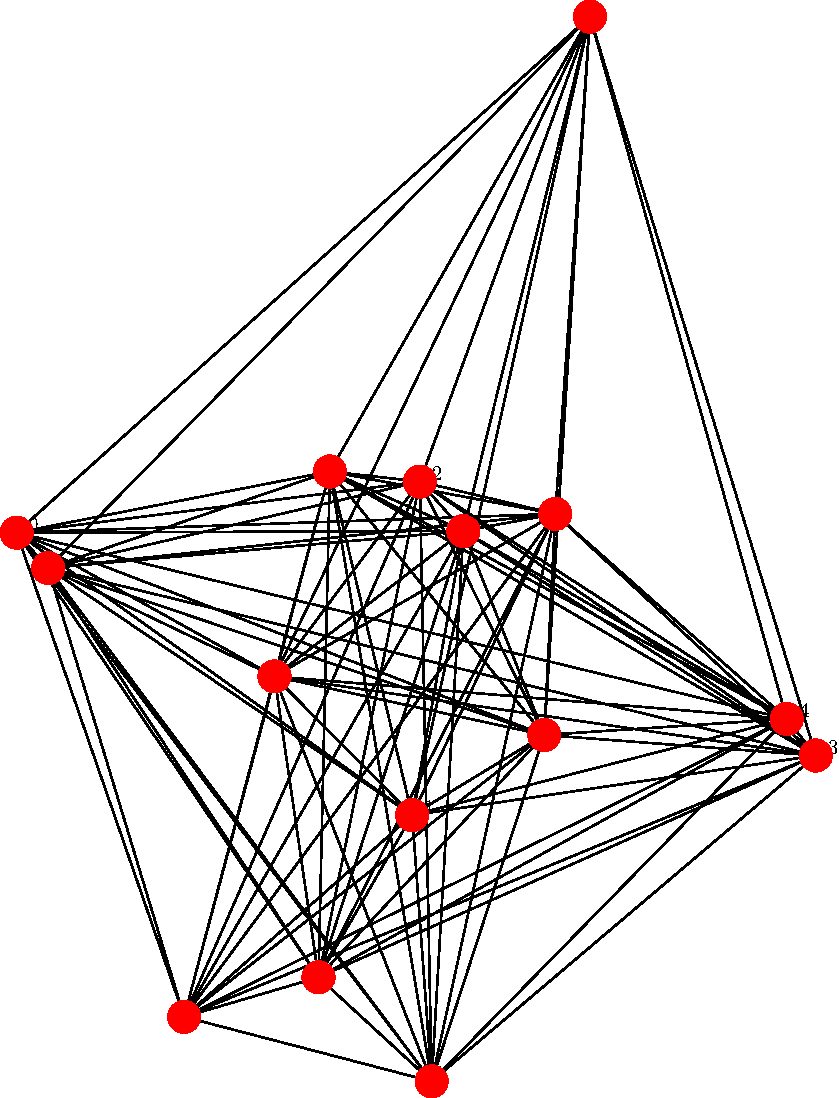
\includegraphics[scale=.25]{smallgraph}
  \caption{Edge graph of the Newton polytope of $\frakX(F_3,\SL(2,\bbC))$.}
\label{fig:f3-sl2c}
\end{figure}

\bibliographystyle{acm}
\bibliography{trop-charvar}
\end{document}

%%% Local Variables:
%%% mode: latex
%%% TeX-master: t
%%% End:
